\documentclass{ucb}

\begin{document}

\ucbcourse{\textbf{ASEN 5331} CFD Unstructured Grid}
\ucbtitle{Final Project Report}
% \ucbgroup{X}
% \ucbdate{15}{09}{2019}
\ucbauthors{
    Pol Mesalles Ripoll \\
}
\ucblocation{Boulder, Colorado}
\ucbcover

\section{Introduction}

The main goal of this project is to implement \textbf{\textit{slip} boundary conditions} into the PHASTA codebase in order to improve the accuracy with which it predicts the flow behavior in the continuum-transition or transitional regime (see \autoref{fig:bird}). Both velocity slip and temperature jump occur when the flow is rarefied enough that the no-slip condition ---taken for granted in most continuum problems--- stops being applicable.

According to previous studies \cite{boydSlip, evaluation}, adding this new capability should increase the fidelity when running simulations at higher Knudsen numbers, as is common in both hypersonics during spacecraft planetary (re)entry, for example, as well as microfluidics, giving results closer to experimental data and simulations conducted with particulate methods, such as the Direct Simulation Monte Carlo (DSMC), which has traditionally been the default choice when studying the continuum-transition. The latter is based on the more generally applicable Boltzmann equation, and thus takes into account non-equilibrium effects. However, especially at lower altitudes, or more generally the lower end of the transitional regime, DSMC simulations can be significantly more computationally expensive than their continuum counterparts, since the number of particles to be simulated increases as Knudsen decreases.

Therefore, there is still a place for CFD solvers based on solving the continuum Navier--Stokes transport equations in the study of the transitional regime. With this project, we seek to implement features that can help PHASTA deliver the same quality of results expected from DSMC, but at a lower cost.

\begin{figure}[H]
    \centering
    \includegraphics[width = 0.8\textwidth]{img/continuum_transition.pdf}
    \caption{The Knudsen number limits on the mathematical models (reproduced from \cite{bird})}
    \label{fig:bird}
\end{figure}

In order to complete this project, this document starts by introducing the different slip models. This is followed by a comprehensive overview of the finite element formulation implemented in PHASTA, along with details about each subroutine in the code. Then, we move on to the specifics about the present implementation of slip boundary conditions. Finally, the results obtained are presented and future relevant work is discussed.

The described changes in the code are available on GitHub, published under the \texttt{slip} branch of my fork of the \texttt{phasta} repository: \url{https://github.com/polmes/phasta/tree/slip}.

\pagebreak

\section{Slip boundary conditions}
\label{sec:slip}

Several slip boundary conditions have been proposed over the years. However, the most common form found in the literature is Maxwell's 1D velocity slip \cite{maxwell, boydSlip}:
\begin{equation}
    u_\mathrm{slip} \equiv u_r = A\left(\frac{2-\sigma}{\sigma}\right)\lambda\left.\frac{\partial u_r}{\partial x_s}\right|_w + \frac{3}{4}\frac{\mu}{\rho T}\frac{\partial T}{\partial x_r}
    \label{eq:maxwell}
\end{equation}
where, in natural coordinates $\left\{r, s, t\right\}$:
\begin{itemize}
    \item $u_\mathrm{slip}$ is the fluid velocity at the surface, assuming a fixed wall.
    \item $A$ is a constant of proportionality, usually taken as $1$.
    \item $\sigma$ is the tangential momentum accommodation coefficient, which basically relates the amount of molecules that are reflected diffusively ($\sigma = 1$) and specularly ($\sigma = 0$).
    \item $\lambda$ is the mean free path, which can be computed from macroscopic properties of the flow as $\lambda = \frac{\mu}{\rho}\sqrt{\frac{\pi}{2RT}}$.
    \item $u_r$ is the velocity in the tangential direction of the wall.
    \item $s$ is the direction normal to the wall.
\end{itemize}

There is also a generalized version of \autoref{eq:maxwell}, which directly relates the slip velocity with the stress tensor and the heat flux \cite{lockerbyVelocity}:
\begin{equation}
    \bm{u}_\mathrm{slip} - \bm{u}_\mathrm{wall} = A\left(\frac{2-\sigma}{\sigma}\right)\frac{\lambda}{\mu}\,\bm{\tau}_{ws} - \frac{3}{4}\frac{\mu}{\rho T}\,\bm{q}_{ws}
    \label{eq:generalized}
\end{equation}
where the subscript $ws$ indicates the shear stress and heat fluxes at the wall in its tangential directions. Relating the stress tensor and heat flux with the velocity and temperature through the constitutive relations used in Navier--Stokes allows us to find more complete expressions for the velocity slip that take into account the surface curvature, which is what we want for a 3D CFD solver \cite{evaluation, newSmoluchowski}.

Besides the velocity slip, another effect related to the rarefied slip regime is the so-called \textit{temperature jump} boundary condition. The most common form is that proposed by Smoluchowski \cite{evaluation, fluidMicrodevices}:
\begin{equation}
    T_\mathrm{slip} - T_\mathrm{wall} = \frac{2-\alpha}{\alpha}\frac{2\gamma}{\gamma+1}\frac{\lambda}{\mathrm{Pr}}\left.\frac{\partial T}{\partial x_s}\right|_w
    \label{eq:smoluchowski}
\end{equation}
where:
\begin{itemize}
    \item $\alpha$ is the thermal accommodation coefficient, often assumed to be the same as $\sigma$.
    \item $\mathrm{Pr}$ is the Prandtl number, which can be computed as $\mathrm{Pr} = \frac{c_p\mu}{\kappa}$, taking $\kappa$ as the thermal conductivity.
\end{itemize}

The idea behind this project is to build the foundation upon which these new boundary conditions can be incorporated into PHASTA, and then see how the results compare to the original code.

\pagebreak

\section{Formulation of the finite element method for CFD}
\label{sec:formulation}

PHASTA solves the compressible Navier--Stokes equations. Starting with the conservative form:
\begin{equation}
    \bm{U}_{,t} + \bm{F}_{i,i} = \bm{\mathcal{F}}
    \label{eq:ns}
\end{equation}
where $\bm{U}$ is the solution vector, $\bm{F}_i$ is the flux vector, and $\bm{\mathcal{F}}$ represents the source term, such that:
\begin{equation}
    \bm{U} =
     \begin{Bmatrix}
        U_1 \\
        U_{j+1} \\
        U_5
    \end{Bmatrix}
    =
    \begin{Bmatrix}
        \rho \\
        \rho u_j \\
        \rho e_\mathrm{tot}
    \end{Bmatrix}
    \qquad
    \bm{F}_i =
    \underbrace{
        \begin{Bmatrix}
            \rho u_i \\
            \rho u_i u_j \\
            \rho u_i e_\mathrm{tot}
        \end{Bmatrix}
        +
        \begin{Bmatrix}
            0 \\
            p\,\delta_{ij} \\
            u_i p
        \end{Bmatrix}
    }_{\bm{F}_i^\mathrm{adv}}
    +
    \underbrace{
        \begin{Bmatrix}
            0 \\
            \tau_{ij} \\
            u_j\tau_{ij}
        \end{Bmatrix}
        +
        \begin{Bmatrix}
            0 \\
            0_j \\
            q_i
        \end{Bmatrix}
    }_{\bm{F}_i^\mathrm{diff}}
\end{equation}
with $e_\mathrm{tot} = e + \frac{1}{2}u_lu_l$, the total energy, $e = c_vT$, the internal energy, $\tau_{ij} = \mu\left(u_{i,j} + u_{j,i}\right) + \lambda u_{l,l}\delta_{ij}$, the viscous stress tensor, and $q_i = -\kappa T_{,i}$, the heat flux according to Fourier's law.

Since the code uses the finite element method, the next step is to find the weak form of \autoref{eq:ns}:
\begin{equation}
    \int_\Omega\left[\bm{W}\cdot\bm{U}_{,t} - \bm{W}_{,i}\cdot\bm{F}_i - \bm{W}\cdot\bm{\mathcal{F}}\right] + \int_\Gamma \bm{W}\cdot\bm{F}_i n_i \, d\Gamma = 0
    \label{eq:global}
\end{equation}
which we get after moving everything to one side (residual form), integrating by parts (over the whole domain $\Omega$ and its boundary $\Gamma$), and multiplying by the weight space functions. 

Since we seek a discrete form of the equations with $n_n$ nodes in the domain, in the Galerkin formulation we use the same shape functions (or basis functions, typically piecewise polynomials) to interpolate both the solution and the weights from nodal values (at $\bm{x}$ locations) as follows:
\begin{subequations}
    \begin{equation}
        \bm{Y}(\bm{x}) = \sum_{A = 1}^{n_n} N_A(\bm{x})\,\bm{Y}_A \qquad \bm{Y}_{,i}(\bm{x}) = \sum_{A = 1}^{n_n}N_{A,i}(\bm{x})\,\bm{Y}_A \qquad \bm{Y}_{,t}(\bm{x}) = \sum_{A = 1}^{n_n} N_A(\bm{x})\,\bm{Y}_{A,t}
    \end{equation}
    \begin{equation}
        \bm{W}(\bm{x}) = \sum_{B = 1}^{n_n} N_B(\bm{x})\,\bm{W}_B \qquad \bm{W}_{,i}(\bm{x}) = \sum_{B = 1}^{n_n} N_{B,i}(\bm{x})\,\bm{W}_B
    \end{equation}
\end{subequations}
where we have replaced $\bm{U}$, the conservative variables, with the array of primitive variables:
\begin{equation}
    \bm{Y} =
    \begin{Bmatrix}
        Y_1 \\
        Y_{j+1} \\
        Y_5
    \end{Bmatrix}
    =
    \begin{Bmatrix}
        p \\
        u_j \\
        T
    \end{Bmatrix}
\end{equation}

In order to evaluate the global integral in the residual above \eqref{eq:global}, we will break it down into a sum of local or element-level integrals, where the solution is now expressed as:
\begin{equation}
    \bm{Y}(\bm{x}) = \sum_{a = 1}^{n_{en}} N_a(\bm{x})\,\bm{Y}_a \qquad \bm{Y}_{,i}(\bm{x}) = \sum_{a = 1}^{n_{en}} N_{a,i}(\bm{x})\,\bm{Y}_a \qquad \bm{Y}_{,t}(\bm{x}) = \sum_{a = 1}^{n_{en}} N_a(\bm{x})\,\bm{Y}_{a,t}
\end{equation}
where $n_{en}$ counts the number of nodes on each element ($a$).It is worth noting that instead of computing the shape functions in physical or real space ($\bm{x}$ coordinates), a better approach is to localize them to the parent or parametric space:
\begin{equation}
    \bm{x}(\bm{\xi}) = \sum_{a = 1}^{n_{en}} N_a(\bm{\xi})\,\bm{x}_a^e \qquad \bm{x}_{\bm{\xi}} = \sum_{a = 1}^{n_{en}} N_{a,\bm{\xi}}(\bm{\xi})\,\bm{x}_a^e
\end{equation}
where $\bm{\xi}$ is a reference coordinate that takes values the same value for every element (from now on indicated by superscript $e$).

The real space gradient of the shape functions can now be evaluated with the chain rule:
\begin{equation}
    N_{a,i}(\bm{\xi}) = N_{a,\xi_j}\xi_{j,i}
    \label{eq:chainrule}
\end{equation}

Putting all these results together, we can rewrite the residual equation \eqref{eq:global} at the element level:
\begin{equation}
    \bm{G}_b^e \equiv \int_\Box \left\{N_b(\bm{\xi})\left[\bm{A}_0\sum_{a = 1}^{n_{en}} N_a(\bm{\xi})\,\bm{Y}_{a,t} - \bm{\mathcal{F}}\right] - N_{b,i}(\bm{\xi})\,\bm{F}_i\right\} D(\bm{\xi}) \, d\Box + \int_{\Box_\Gamma} N_b(\bm{\xi})\,\bm{F}_i n_i \, D_\Gamma(\bm{\xi}) \, d\Box_\Gamma
    \label{eq:local}
\end{equation}
where $\bm{A}_0$ relates the primitive and conservative variables, $D(\bm{\xi}) \equiv \det(\bm{x}_{\bm{\xi}})$ is the Jacobian of the coordinate transformation, and the symbol $\Box$ is used to denote the reference space.

Since we want to evaluate the integrals in \autoref{eq:local} in an efficient manner, we will make use of Gauss quadrature in the parent domain:
\begin{equation}
    \int_\Box f(\bm{\xi}) \, d\Box \approx \sum_{k = 1}^{n_\mathrm{int}} f(\bm{\xi}^k) \, w^k
\end{equation}
where $\bm{\xi}^k$ and $w^k$ are, respectively, the position and weight ---in parametric coordinates--- of the $n_\mathrm{int}$ quadrature points, which can change depending on the order of integration.

Finally, the $n_e$ elemental residuals computed with \eqref{eq:local} are assembled together to recover the global residual we seek:
\begin{equation}
    \bm{G}_B = \Assembly_{e=1}^{n_e} \bm{G}_b^e = 0
\end{equation}

The Galerkin method that has been presented so far is shown to be unstable for convection-dominated flows. Hence, we add an additional stabilization term to the residual:
\begin{equation}
    \bm{\hat{G}}_b^e = \underbrace{\bm{G}_b^e}_{\text{Galerkin}} + \underbrace{\int_\Box \hat{\mathcal{L}}\,N_b(\bm{\xi}) \cdot \bm{\tau}\left[\mathcal{L}\bm{Y} - \bm{\mathcal{F}}\right] D(\bm{\xi}) \, d\Box}_{\text{Stabilization}}
\end{equation}
where the following "least squares" linear operator is defined:
\begin{equation}
    \mathcal{L} \equiv \bm{A}_0\,\frac{\partial}{\partial t} + \bm{A}_i\,\frac{\partial}{\partial x_i} - \frac{\partial}{\partial x_i}\left[\bm{K}_{ij}\frac{\partial}{\partial x_j}\right]
\end{equation}
with the matrices above being such that the following relations hold true:
\begin{equation}
    \bm{A}_0 \equiv \bm{U}_{,\bm{Y}} \qquad {A}_i \equiv \bm{F}_{i,\bm{Y}}^\mathrm{adv} \qquad \bm{F}_i^\mathrm{diff} = -\bm{K}_{ij} \bm{Y}_{,j}
\end{equation}
and hence when the operator is applied to the solution vector, the result is simply the original LHS of the Navier--Stokes strong form \eqref{eq:ns}:
\begin{equation}
    \mathcal{L}\bm{Y} = \bm{A}_0\bm{Y}_{,t} + \bm{A}_i\bm{Y}_{,i} - \left[\bm{K}_{ij} \bm{Y}_{,j}\right]_{,i} = \bm{U}_{,t} + \bm{F}_{i,i}^\mathrm{adv} + \bm{F}_{i,i}^\mathrm{diff}
\end{equation}
showing that the added stabilization term is just a residual that disappears when the solution converges.

Additionally, the operator $\hat{\mathcal{L}}$, which together with the $\bm{\tau}$ matrix of timescales act as a weight to this additional residual, can take different forms. In Streamline Upwind Petrov--Galerkin (SUPG), the scheme used by PHASTA, it is defined to only consider advection:
\begin{equation}
    \hat{\mathcal{L}} \equiv \bm{A}_{i}\,\frac{\partial}{\partial x_i}
\end{equation}

At this point, the FEM spatial discretization has allowed us to transform the original partial differential equation \eqref{eq:ns} into the residual $\bm{\hat{G}}_B(\bm{Y},\bm{Y}_{,t})$ of a nonlinear system of ordinary differential equations. Next, we will use a generealized-$\alpha$ time integrator to turn this into a nonlinear system of algebraic equations:
\begin{subequations}
    \begin{align}
        &\overset{n+1}{\bm{Y}_A^{(i)}} = \overset{n}{\bm{Y}_A} + \Delta t \, \overset{n}{\bm{Y}_{A,t}} + \Delta t \left[\overset{n+1}{\bm{Y}_{A,t}^{(i)}} - \overset{n}{\bm{Y}_{A,t}}\right] &\forall \ A
        \label{eq:od1}
        \\
        &\bm{\hat{G}}_B\left(\overset{n+\alpha_m}{\bm{Y}_{A,t}^{(i)}}, \overset{n+\alpha_f}{\bm{Y}_A^{(i)}}\right) = 0 &\forall \ B
        \label{eq:od2}
        \\
        &\overset{n+\alpha_m}{\bm{Y}_{A,t}^{(i)}} = \overset{n}{\bm{Y}_{A,t}} + \alpha_m \left[\overset{n+1}{\bm{Y}_{A,t}^{(i)}} - \overset{n}{\bm{Y}_{A,t}}\right] &\forall \ A
        \label{eq:od3}
        \\
        &\overset{n+\alpha_f}{\bm{Y}_A^{(i)}} = \overset{n}{\bm{Y}_A} + \alpha_f \left[\overset{n+1}{\bm{Y}_A^{(i)}} -  \overset{n}{\bm{Y}_A}\right] &\forall \ A
        \label{eq:od4}
    \end{align}
\end{subequations}
where $i$ is the time iteration and counter, and the parameters $\alpha_f$ and $\alpha_m$ are not necessarily equal. Given a $\rho_\infty$ amplification factor, for second order accuracy in time these can be selected as follows:
\begin{equation}
    \alpha_m = \frac{1}{2}\left[\frac{3 - \rho_\infty}{1 + \rho_\infty}\right] \qquad
    \alpha_f = \frac{1}{1 + \rho_\infty} \qquad
    \gamma = \frac{1}{2} + \alpha_m - \alpha_f
\end{equation}

Newton's method is used to linearize the algebraic system of equations such that in each iteration we can find the difference in our solution needed for the residual to become zero. We choose to linearize about $\overset{n+\alpha_f}{\bm{Y}_A^{(i)}}$, resulting in the followin linear system of equations:
\begin{equation}
    \underbrace{\bm{\hat{G}}_B\left(\overset{n+\alpha_m}{\bm{Y}_{A,t}^{(i)}}, \overset{n+\alpha_f}{\bm{Y}_A^{(i)}}\right)}_{\bm{R}_B} + \underbrace{\sum_{A = 1}^{n_n} \frac{\partial\overset{\mathrm{LHS}}{\bm{G}_B}}{\partial\overset{n+\alpha_f}{\bm{Y}_A^{(i)}}}}_{\bm{M}_{BA}}\,\underbrace{\Delta\overset{n+\alpha_f}{\bm{Y}_A^{(i)}}}_{\Delta\bm{Y}_A} = \bm{0}
    \label{eq:newton}
\end{equation}
where $\bm{R}_B$ is the RHS residual, $\bm{M}_{BA}$ is called the LHS tangent or mass matrix, and $\Delta\overset{n+\alpha_f}{\bm{Y}_A^{(i)}}$ is the difference we seek. Note that the tangent matrix is computed at the element level and then assembled globally.

Furthermore, the LHS residual is computed differently for better convergence, reversing integration by parts on the advective term and dropping the boundary integral:
\begin{equation}
    \overset{\mathrm{LHS}}{\bm{G}_b} = \int_\Box \left\{ N_b\left[\bm{A}_0 \, \overset{n+\alpha_m}{\bm{Y}_{a,t}^{(i)}} + \bm{A}_i \, \overset{n+\alpha_f}{\bm{Y}_{a,i}^{(i)}} - \bm{\mathcal{F}}\right] + N_{b,i} \, \bm{K}_{ij} \, \overset{n+\alpha_f}{\bm{Y}_{a,j}^{(i)}} + \hat{\mathcal{L}}\,N_b \cdot \bm{\tau}\left[\bm{A}_0 \, \overset{n+\alpha_m}{\bm{Y}_{a,t}^{(i)}} + \bm{A}_i \, \overset{n+\alpha_f}{\bm{Y}_{a,i}^{(i)}} - \bm{\mathcal{F}}\right]\right\} D(\bm{\xi}) \, d\Box
\end{equation}

\pagebreak

Using a predictor/multi-correct iteration process, the following algorithm is applied inside a loop over timesteps:
\begin{enumerate}
    \item Set initial values for $\overset{n+1}{\bm{Y}_A^{(i)}}$ with data from the previous timestep or initial conditions.
    \label{startstart}
    \item Solve \autoref{eq:od1} to get a consistent prediction of $\overset{n+1}{\bm{Y}_{A,t}^{(i)}}$.
    \item Interpolate the solution vector $\overset{n+\alpha_f}{\bm{Y}_A^{(i)}}$ and its derivative $\overset{n+\alpha_m}{\bm{Y}_{A,t}^{(i)}}$ with the selected parameters using \eqref{eq:od3} and \eqref{eq:od4}.
    \item Compute the residual $\bm{\hat{G}}_B$ with \autoref{eq:od2}.
    \label{loopstart}
    \item Using Newton's method \eqref{eq:newton}, find the difference $\Delta\overset{n+\alpha_f}{\bm{Y}_A^{(i)}}$ that makes the residual zero.
    \item Update our solution vectors: $\overset{n+\alpha_f}{\bm{Y}_A^{(i+1)}} = \overset{n+\alpha_f}{\bm{Y}_A^{(i)}} + \Delta\overset{n+\alpha_f}{\bm{Y}_A^{(i)}}$, and find $\overset{n+\alpha_m}{\bm{Y}_{A,t}^{(i+1)}}$ with \eqref{eq:od1} and \eqref{eq:od4}.
    \label{loopend}
    \item Keep iterating \ref{loopstart}--\ref{loopend} until the residual drops below a specified tolerance, the solution difference goes below a secondary tolerance, or the maximum number of iterations per timestep is reached.
    \item Move to the next timestep, starting back again at \ref{startstart}.
\end{enumerate}

The compressible version of PHASTA has multiple ways to approach the solution of the linear system of equations presented in \autoref{eq:newton}, all of which are based on the iterative method known as generalized minimal residual (GMRES), since for large problems direct solvers are not possible.

Before we discuss the possible approaches, we must first introduce preconditioning. CFD problems are notoriously ill-conditioned, an issue that originates with the scales of the different terms in the Navier--Stokes equations ($p$, $u$, and $T$ all have different orders of magnitude). In PHASTA, before solving the system we will make use of symmetric block-diagonal preconditioning. Start by defining:
\begin{equation}
    \bm{B} \equiv \diag\left(\bm{M}_{BA}\right)
\end{equation}
and then, using the Cholesky method, we can decompose the above into the product of a lower triangular matrix $\bm{L}$ and an upper triangular matrix $\bm{U}$. With these, we see better results by modifying the the original system of equations as follows:
\begin{equation}
    \underbrace{\bm{L}^{-1} \bm{M}_{BA} \bm{U}^{-1}}_{\bm{A}} \, \underbrace{\bm{U} \Delta\bm{Y}_A}_{\bm{x}} = \underbrace{-\bm{L}^{-1}\bm{R}_B}_{\bm{b}}
\end{equation}
and after finding $\bm{x}$, we can recover the original solution we seek as $\Delta\bm{Y}_A = \bm{U}^{-1}\bm{x}$.

Iterative solvers approximate the solution $\bm{x}$ as $\bm{x}_0 + \bm{z}$, where $\bm{x}_0$ is an initial guess and $\bm{z}$ is iteratively constructed such that the norm $\norm{\bm{A}\left(\bm{x}_0 + \bm{z}\right) - \bm{b}}$ is minimized. GMRES considers $\bm{z}$ to be a member ---that is, a linear combination--- of the Krylov subspace:
\begin{equation}
    \mathcal{K} = \spanspace\left\{\bm{r}_0, \bm{A}\bm{r}_0, \bm{A}^2\bm{r}_0, \ldots, \bm{A}^k\bm{r}_0\right\}
\end{equation}
with $\bm{r}_0 = \bm{A}\bm{x}_0 - \bm{b}$, the error of the initial guess.

Note that each subsequent Krylov vector is the product of the previous one:
\begin{equation}
    \bm{v}_k = \bm{A}^{k-1}\bm{r}_0 = \bm{A}\bm{v}_{k-1} \equiv \bm{A}\bm{p} = \bm{q}
\end{equation}
and is then made orthonormal with respect to all the previous ones.

Recall that so far we have not computed the global $\bm{A}$ (or $\bm{M}_{BA}$) matrix. It is not practical, but we still need to compute the matrix-vector product $\bm{A}\bm{p}$. As mentioned earlier, in PHASTA there are three different approaches:
\begin{enumerate}
    \item Elemen-by-Element GMRES: instead of assembling the elemental $\bm{A}^e$ matrices, we localize the global Krylov vectors:
    \begin{equation}
        \bm{p}^e = \Localize_{e = 1}^{n_e} \bm{p}
    \end{equation}
    and then perform the matrix-vector product at the element level, and assemble the result:
    \begin{equation}
        \bm{q}^e = \bm{A}^e \bm{p}^e \implies \bm{q} = \Assembly_{e = 1}^{n_e} \bm{q}^e
    \end{equation}
    
    \item Matrix-Free GMRES: recall that $\bm{A} = \frac{\partial\bm{G}}{\partial\bm{Y}}$ (dropped indices), and thus can be approximated as:
    \begin{equation}
        \bm{A} \approx \frac{\bm{G}(\bm{Y} + \varepsilon\bm{v}) - \bm{G}(\bm{Y})}{\varepsilon\bm{v}}
    \end{equation}
    where $\varepsilon$ is a perturbation with an arbitrary variable $\bm{v}$ that represents an increment $\Delta\bm{Y}$. Since what we seek is a matrix-vector product, replacing $\bm{v}$ above by $\bm{p}$, we have:
    \begin{equation}
        \bm{A}\bm{p} \approx \frac{\bm{G}(\bm{Y} + \varepsilon\bm{p}) - \bm{G}(\bm{Y})}{\varepsilon\cancel{\bm{p}}}\,\cancel{\bm{p}}
    \end{equation}
    and we see that there is no need to form the $\bm{A}$ matrix, greatly reducing the memory use required.
    
    \item Sparse GMRES: in this case, the $\bm{A}$ matrix is sparsely assembled, meaning that we only store the nonzeros in a stacked array. In this way, when performing the $\bm{A}\bm{p}$ product, the number of floating point operations is minimized.
\end{enumerate}

Finally, we need to discuss how boundary conditions are imposed. These can be of either essential (Dirichlet) or natural (Neumann) types.

When dealing with essential boundary conditions, the value of the unknown is directly specified on the boundary $\Gamma_g$. PHASTA supports the following list of $v^g$ variables to be prescribed at any point:
\begin{equation}
    \begin{Bmatrix}
        p^g \\ u_r^g \\ u_s^g \\ u_t^g \\ T^g \\ \rho^g
    \end{Bmatrix}
    =
    \begin{Bmatrix}
        Y_1 \\ c_i^r Y_{i+1} \\ c_i^s Y_{i+1} \\ c_i^t Y_{i+1} \\  Y_5 \\ \frac{Y_1}{RY_5}
    \end{Bmatrix}
    \label{eq:vg}
\end{equation}
where $c_i^r$, $c_i^s$, and $c_i^t$ represent the direction cosines of the velocity vector $\left(u_r^g, u_s^g, u_t^g\right)$, components usually considered to be aligned with the wall (non-cartesian). Rearranging \autoref{eq:vg}, we can find the $\bm{\hat{q}}$ vector, which modified the values of our solution vector $\bm{Y}$ as a function of the Dirichlet boundary conditions where necessary:
\begin{equation}
    \begin{Bmatrix}
        Y_1 \\ Y_2 \\ Y_3 \\ Y_4 \\ Y_5 \\ Y_1
    \end{Bmatrix}
    =
    \begin{Bmatrix}
        p^g \\
        \frac{1}{c_1^r}\left(u_r^g - c_2^r Y_3 - c_3^r Y_4\right) \\
        \frac{1}{c_2^s}\left(u_s^g - c_1^s Y_2 - c_3^s Y_4\right) \\
        \frac{1}{c_3^t}\left(u_t^g - c_1^t Y_2 - c_2^t Y_3\right) \\
        T^g \\
        \rho^g R Y_5
    \end{Bmatrix}
    \equiv
    \bm{\hat{q}}
    \label{eq:qv}
\end{equation}

PHASTA also has support for periodic boundary conditions, which are similar to Dirichlet in the sense that they directly modify the value of the solution vector. In this case, though, the value is taken to be the same as the solution in a partner node.

Besides modifying the solution vector as shown above, in order to impose essential boundary conditions, we will also need to constraint the weight space such that it fulfills the relations above. For each possible variable $k$, a new weight is derived as follows:
\begin{equation}
    W_k' = \frac{\partial \hat{q}_k}{\partial Y_j}W_j
\end{equation}

In PHASTA, this is implemented by modifying the corresponding $\bm{M}_{BA}$ matrix and $\bm{R}_B$ vector from \autoref{eq:newton} with a matrix $\bm{S}_v$ that relates the old weights with the new ones, $\bm{W}' = \bm{S}_v \bm{W}$ for each possible variable $v^g$. The new system of equations becomes:
\begin{equation}
    \underbrace{\bm{S}_v^T\bm{M}_{BA}\bm{S}_v}_{\bm{\tilde{M}}_{BA}} \, \Delta\bm{Y}_A = -\underbrace{\bm{S}_v^T \bm{R}_B}_{\bm{\tilde{R}}_B}
\end{equation}
which, again, is modified at the element level and then assembled to obtain the global matrix.

As a notable example, when setting the three components of velocity at a given point, the transformation of the weight space is:
\begin{equation}
    \bm{S}_{rst} = 
        \begin{bmatrix}
            1 & 0 & 0 & 0 & 0 \\
            0 & 0 & 0 & 0 & 0 \\
            0 & 0 & 0 & 0 & 0 \\
            0 & 0 & 0 & 0 & 0 \\
            0 & 0 & 0 & 0 & 1
        \end{bmatrix}
\end{equation}

On the other hand, for natural boundary conditions, the flux of the variable is prescribed on a boundary $\Gamma_h$. In this case, the constraints are imposed during the integration of the boundary elements when computing the residual \eqref{eq:local}, as follows:
\begin{multline}
    \begin{aligned}
        \int_{\Box_\Gamma} N_b\left[\bm{F}_i^\mathrm{adv} + \bm{F}_i^\mathrm{diff}\right] n_i \, D \, d\Box_\Gamma &= \int_{\Box_\Gamma} N_b \left[u_n\bm{U} + p\begin{Bmatrix}0 \\ \delta_{jn} \\ u_n\end{Bmatrix} - \begin{Bmatrix}0 \\ \tau_{jn} \\ \tau_{jn} u_j\end{Bmatrix} + \begin{Bmatrix}0 \\ 0_j \\ q_n\end{Bmatrix}\right] D_\Gamma \, d\Box_\Gamma \\
        &= \int_{\Box_{\Gamma_h^m}} N_b \, h^m \, \bm{U} \, D_\Gamma \, d\Box_\Gamma + \int_{\Box_{\Gamma-\Gamma_h^m}} N_b \, u_n \, \bm{U} \, D_\Gamma \, d\Box_\Gamma \\
        &+ \int_{\Box_{\Gamma_h^p}} N_b \, h^p \begin{Bmatrix}0 \\ \delta_{jn} \\ u_n\end{Bmatrix} D_\Gamma \, d\Box_\Gamma + \int_{\Box_{\Gamma-\Gamma_h^p}} N_b \, p \begin{Bmatrix}0 \\ \delta_{jn} \\ u_n\end{Bmatrix} D_\Gamma \, d\Box_\Gamma \\
        &- \int_{\Box_{\Gamma_h^v}} N_b \begin{Bmatrix}0 \\ h_j^v \\ h_j^v u_j\end{Bmatrix} D_\Gamma \, d\Box_\Gamma - \int_{\Box_{\Gamma-\Gamma_h^v}} N_b \begin{Bmatrix}0 \\ \tau_{jn} \\ \tau_{jn} u_j\end{Bmatrix} D_\Gamma \, d\Box_\Gamma \\
        &+ \int_{\Box_{\Gamma_h^h}} N_b \begin{Bmatrix}0 \\ 0_j \\ h_h^h\end{Bmatrix} D_\Gamma \, d\Box_\Gamma + \int_{\Box_{\Gamma-\Gamma_h^h}} N_b \begin{Bmatrix}0 \\ 0_j \\ q_n\end{Bmatrix} D_\Gamma \, d\Box_\Gamma
    \end{aligned}
\end{multline}
where $h^k$ are the prescribed flux values on the boundary $\Gamma_h^k$, and then we have a floating flux on $\Gamma - \Gamma_h^k$, which is computed using the current value of the solution.


% notes on parallel algorithms?


\section{PHASTA codebase}
\label{sec:code}

In this section, we describe how the PHASTA code (compressible version) is implemented, including the main variables and functions used and how they relate to the FEM theory presented so far.

It is worth noting that, since PHASTA is designed to run in parallel, the whole domain is first divided into parts, and each of these is then further divided into blocks of elements. These blocks have a fixed size designed to optimize cache performance in Fortran implicit loops, which are used throughout the code.

\subsection{Summary of variables}

First of all, as many of the variables defined in PHASTA are vectors or matrices, below is a reference of all the dimensions mentioned throughout this document:
\begin{itemize}
    \item \texttt{nsd} is the number of space dimensions (generally 3).
    \item \texttt{npro} is the number of elements to process in a single block call ($n_e$ in the notes).
    \item \texttt{nenl} is the number of vertices per element.
    \item \texttt{nshl} is the local number of shape functions per element (local nodes, $a = 1 \ldots n_{en} $ in the notes).
    \item \texttt{nshg} the global number of shape functions (total number of nodes, $A = 1 \ldots n_n$ in the notes).
    \item \texttt{ngauss} is the number of Gauss quadrature integration points in an element ($n_{\mathrm{int}}$ in the notes).
    \item \texttt{nflow} is the number of flow variables in the solution vector (5 in the compressible 3D case).
    \item \texttt{ndof} is the number of degrees of freedom per node (basically, \texttt{ndof = nflow + scalars}).
    \item \texttt{nedof = nflow * nshl} is the total number of degrees of freedom at each element node.
    \item \texttt{nnz\_tot} is the total number of nonzeros in the LHS matrix.
    % \item \texttt{ndofBC = ndof + 1} is the size of the \texttt{BC} array.
    \item \texttt{nshlb} is like \texttt{nshl}, but for the boundary elements.
    \item \texttt{ngaussb} is like \texttt{ngauss}, but for the boundary elements.
    \item \texttt{nenbl} is the number of nodes in a boundary face for the boundary elements.
    \item \texttt{Kspace} is the dimension of the Krylov subspace.
    \item \texttt{nlwork} is the size of the array local to the processor.
\end{itemize}

Some of these variables are stored per each \texttt{iblk} block of elements for ease of access in the \texttt{lcblk} array, as detailed below:
\begin{itemize}
    \item \texttt{lcblk(1,iblk) = iel} is the element counter, and is used to compute the number of elements in the block as \texttt{npro = lcblk(1,iblk+1) - iel}.
    \item \texttt{lcblk(3,iblk) = lcsyst} represents the element topology in the block (\texttt{1} for tetrahedrons, \texttt{2} for hexahedrons, \texttt{3} for wedges, \texttt{5} for pyramids).
    \item \texttt{lcblk(4,iblk) = iorder} is the element order
    \item \texttt{lcblk(5,iblk) = nenl}.
    \item \texttt{lcblk(10,iblk) = nshl}.
\end{itemize}

\autoref{tab:vars} summarizes the most important variables used throughout the PHASTA code and their correspondence with the theory covered in \autoref{sec:formulation}.

\pagebreak

\begin{longtable}[c]{m{0.3\textwidth} m{0.15\textwidth} m{0.46\textwidth}}
    \caption{List of the main variables (and their dimensions) used in PHASTA}
    \label{tab:vars}
    \\
    
    \toprule
    \textbf{In code} & \textbf{In the notes} & \textbf{Description} \\
    \midrule
    \midrule
    \endfirsthead
    \toprule
    \textbf{In code} & \textbf{In the notes} & \textbf{Description} \\
    \midrule
    \midrule
    \endhead
    
    \texttt{y(nshg,ndof)} & $\overset{n+\alpha_f}{\bm{Y}^{(i)}}$ & Solution array (primitive global variables) at current timestep. Their order is $\{u_j, p, T\}$. \\
    \midrule
    \texttt{x(nshg,nsd)} & $\bm{x}$ & Global node (vertex) coordinates. \\
    \midrule
    \texttt{ac(nshg,ndof)} & $\overset{n+\alpha_m}{\bm{Y}_{,t}^{(i)}}$ & Acceleration array (time derivative of solution vector). \\
    \midrule
    \texttt{yold(nshg,ndof)} & $\overset{n}{\bm{Y}}$ & Solution vector at previous (or initial) timestep. \\
    \midrule
    \texttt{acold(nshg,ndof)} & $\overset{n}{\bm{Y}_{,t}}$ & Acceleration vector at previous (or initial) timestep. \\
    \midrule
    \texttt{shp(nshl,ngauss)} & $N_a$ & Element shape functions evaluated at the quadrature points. In the code, this is sometimes referred to as \texttt{shape}, and is then reshaped to be of the form \texttt{shp(npro,nshl)} for each Gauss point. \\
    \midrule
    \texttt{shgl(nsd,nshl,ngauss)} & $N_{a,\bm{\xi}}$ & Element local shape function gradients (in the parent domain) evaluated at the quadrature points. In the code, this is sometimes referred to as \texttt{shdrv}, and is then reshaped to be of the form \texttt{shgl(npro,nsd,nshl)} for each Gauss point. \\
    \midrule
    \texttt{shg(npro,nshl,nsd)} & $N_{a,i}$ & Global gradient of element shape functions. \\
    \midrule
    \texttt{dxdxi(npro,nsd,nsd)} & $\bm{x}_{,\bm{\xi}}$ & Jacobian of the map from real domain to parent domain. \\
    \midrule
    \texttt{dxidx(npro,nsd,nsd)} & $\bm{\xi}_{,i} = \xi_{j,i}$ & Inverse of the above, the metric tensor that maps the parent domain to the real domain. \\
    \midrule
    \texttt{WdetJ(npro)} & $w^k D(\bm{\xi}^k)$ & Weighted Jacobian for spatial (quadrature) integration. \\
    \midrule
    \texttt{ien(npro,nshl)} & -- & Nodal connectivity matrix that given \texttt{element \#, local node \#} returns the \texttt{global node \#}. \\
    \midrule
    \texttt{yl(npro,nshl,nflow)} & $\overset{n+\alpha_f}{\bm{Y}_a}$ & Solution array (primitive variables) at current timestep. Their order is $\{p, u_j, T\}$. \\ \\
    \midrule
    \texttt{ycl(npro,nshl,ndof)} & -- & Corresponds to a vector with $\overset{n+\alpha_f}{\bm{Y}_a}$ and scalars. \\
    \midrule
    \texttt{acl(npro,nshl,ndof)} & $\overset{n+\alpha_m}{\bm{Y}_{a,t}}$ & Acceleration vector at current timestep. \\
    \midrule
    \texttt{xl(npro,nshl,nsd)} & $\bm{x}_a^e$ & Local node coordinates. \\
    \midrule
    \texttt{dui(npro,nflow)} & $\Delta\overset{n}{\bm{U}}$ & Delta of conservative variables at previous timestep. \\
    \midrule
    \texttt{pres} & $p$ & Pressure at the quadrature point. \\
    \midrule
    \texttt{u1}, \texttt{u2}, \texttt{u3} & $u_j$ & Velocity (in the $j$ direction) at the quadrature point. \\
    \midrule
    \texttt{T} & $T$ & Temperature at the quadrature point. \\
    \midrule
    \texttt{g1yi(npro,nflow), g2yi(npro,nflow), g3yi(npro,nflow)} & $\bm{Y}_{,i}$ & Gradient of the solution vector. \\
    \midrule
    \texttt{A0(npro,nflow,nflow)} & $\bm{A}_0 = \bm{U}_{,\bm{Y}}$ & Matrix that maps conservative variables to primitive variables. \\
    \midrule
    \texttt{A1(npro,nflow,nflow), A2(npro,nflow,nflow), A3(npro,nflow,nflow)} & $\bm{A}_i = \bm{F}_{i,\bm{Y}}^\mathrm{adv}$ & Matrices that relate the divergence of the advective flux such that $\bm{F}_{i,i}^\mathrm{adv} = \bm{A}_i \bm{Y}_{,i}$. \\
    \midrule
    \texttt{stiff(npro,nsd*nflow,} \texttt{nsd*nflow)} & $\bm{K}_{ij}$ & Diffusive tangent matrix such that the viscous flux can be computed as $\bm{F}_i^\mathrm{diff} = -\bm{K}_{ij} \bm{Y}_{,j}$. \\
    \midrule
    \texttt{tau(npro,3)} & $\bm{\tau}$ & Stabilization matrices (continuity, momentum, energy). \\
    \midrule
    \texttt{src(npro,nflow)} & \bm{\mathcal{F}} & Body force vector. \\
    \midrule
    \texttt{ri(npro,nflow*(nsd+1)} & -- & Partial residual. \texttt{ri(:,1:15} represents $\bm{F}_i = \bm{F}_i^\mathrm{adv} + \bm{F}_i^\mathrm{diff}$, while \texttt{ri(16:20)} collects $\bm{A}_0\bm{Y}_{,t} - \bm{\mathcal{F}}$. \\
    \midrule
    \texttt{rLyi(npro,nflow)} & $\mathcal{L}\bm{Y} - \bm{\mathcal{F}}$ & Least-squares residual vector, where the operator $\mathcal{L} \equiv \bm{A}_0\frac{\partial}{\partial t} + \bm{A}_i\frac{\partial}{\partial x_i} - \frac{\partial}{\partial x_i}\left(\bm{K}_{ij}\frac{\partial}{\partial x_j}\right)$ is used. \\
    \midrule
    \texttt{rl(npro,nshl,nflow)} & $\bm{\hat{G}}_b^e$ & Element-level residual. \\
    \midrule
    \texttt{res(nshg,nflow)} & $\bm{\hat{G}}_B$ & Global residual. \\
    \midrule
    \texttt{EGmass(npro,nedof,nedof)} & $\bm{M}_{ba} = \bm{\hat{G}}_{b,\bm{Y}_a}$ & Element-level LHS tangent mass matrix. \\
    \midrule
    \texttt{lhsK(nflow*nflow,nnz\_tot)} & $\bm{M}_{BA}$ & Sparsely assembled LHS mass matrix. \\
    \midrule
    \texttt{iBC(nshg)} & -- & Essential boundary condition binary code. The code currently goes up to $2^{13}$, where each digit represents whether a condition is prescribed or not (e.g., $10101010101010$), and they are ordered as follows: density ($2^0$), temperature ($2^1$), pressure ($2^2$), velocity components ($x_1$, $2^3$; $x_2$, $2^4$; $x_3$, $2^5$), scalars ($2^6$, $2^7$, $2^8$, $2^9$), periodicity ($2^{10}$), SPEBC ($2^{11}$), axisymmetric ($2^{12}$), and wall deformation ($2^{13}$). \\
    \midrule
    \texttt{BC(nshg,ndof+1)} & $\bm{\hat{q}} = f(p^g, u_j^g, T^g, \rho^g)$ & Essential boundary condition constraint parameters. Includes prescribed values for density, pressure, temperature, and velocity, as well as the corresponding direction consine terms. \\
    \midrule
    \texttt{iBCB(npro,2)} & -- & Natural boundary condition code, equivalent to \texttt{iBC}. In this case, the order of \texttt{iBCB(:,1)} is: convective flux ($2^0$), pressure flux ($2^1$), viscous flux ($2^2$), heat flux ($2^3$), turbulence wall ($2^4$), and the next are scalar fluxes. \texttt{iBCB(:,2)} is the \texttt{srfID} given by the user for which the integrated fluxes will be colleted. \\
    \midrule
    \texttt{BCB(npro,nshlb,ndof+1)} & $h^k(\bm{x})$ & Natural boundary condition prescribed fluxes. \\
    \midrule
    \texttt{xlb(npro,nenl,nsd)} & $x_b^e$ & Like \texttt{xl}, but for boundary elements. \\
    \midrule
    \texttt{shpb(nshl,ngaussb)} & $N_b$ & Like \texttt{shp}, but for boundary elements. Reshaped to \texttt{shpb(npro,nshl)} for each Gauss point. \\
    \midrule
    \texttt{shglb(nsd,nshl,ngaussb)} & $N_{b,\bm{\xi}}$ & Like \texttt{shgl}, but for boundary elements. Reshaped to \texttt{shglb(npro,nsd,nshl)} for each Gauss point. \\
    \midrule
    \texttt{dxdxib(npro,nsd,nsd)} &  $\bm{x}_{,\bm{\xi}}$ & Like \texttt{dxdxi}, but for boundary elements. \\
    \midrule
    \texttt{dxidxb(npro,nsd,nsd)} & $\bm{\xi}_{,i} = \xi_{j,i}$ & Like \texttt{dxidx}, but for boundary elements. \\
    \midrule
    \texttt{WdetJb(npro)} & $w^k D_\Gamma(\bm{\xi}^k)$ & Like \texttt{WdetJ}, but for boundary elements. \\
    \midrule
    \texttt{bnorm(npro,nsd)} & $\bm{\hat{n}}$ & Outward normal vector (to the surface). \\
    \midrule
    \texttt{rou(npro)} & $h^m\bm{U}$ & Boundary condition mass flux. \\
    \midrule
    \texttt{p(npro)} & $h^p\begin{Bmatrix}0 \\ \delta_{jn} \\ u_n\end{Bmatrix}$ & Boundary condition natural pressure. \\
    \midrule
    \texttt{tau1n(npro)}, \texttt{tau2n(npro)}, \texttt{tau3n(npro)} & $\begin{Bmatrix}0 \\ h_j^v \\ h_j^v u_j\end{Bmatrix}$ & Boundary condition viscous flux. \\
    \midrule
    \texttt{heat(npro)} & $\begin{Bmatrix}0 \\ 0_j \\ h^h\end{Bmatrix}$ & Boundary condition heat flux. \\
    \midrule
    \texttt{F1(npro)}, \texttt{F2(npro)}, \texttt{F3(npro)}, \texttt{F4(npro)}, \texttt{F5(npro)} & $\bm{F}_i n_i$ & Total flux normal to the boundary. \\
    \midrule
    \texttt{Force(3)} & -- & 3 components of the integrated aerodynamic forces on the body. \\
    \midrule
    \texttt{Hflux} & -- & Total integrated heat flux on the body. \\
    \midrule
    \texttt{iper(nshg)} & -- & Partners of periodic boundary conditions,relates the master node to the slave node so that they end up having the same values. \\
    \midrule
    \texttt{BDiag(nshg,nflow,nflow)} & $\bm{B}$ & Block-diagonal preconditioner matrix. \\
    \midrule
    \texttt{Dy(nshg,nflow)} & $\Delta\overset{n+\alpha_f}{\bm{Y}_A^{(i)}}$ & Difference in solution vector. \\
    \midrule
    \texttt{uBrg(nsh,nflow,Kspace+1)} & $\bm{v}_k$ & Krylov vector. \\
    \midrule
    \texttt{HBrg(Kspace+1,Kspace)} & -- & Upper Hessenberg matrix. \\
    \midrule
    \texttt{eBrg(Kspace+1)} & $\norm{\bm{A}\left(\bm{x}_0 + \bm{z}\right) - \bm{b}}$ & Error of the minimization problem in GMRES. \\
    \midrule
    \texttt{yBrg(Kspace)} & $\bm{x}_0 + \bm{z}$ & Solution of the minimization problem in GMRES. \\
    \midrule
    \texttt{row(nnz*nshg)} & -- & Helper array that collects in a stacked structure all the nonzeros in a given row (according to the links between nodes). \\
    \midrule
    \texttt{col(nshg+1)} & -- & Helper array that determines what on what index of \texttt{row} each new row starts. Its size is \texttt{nshg+1} to indicate the end point. \\
    \midrule
    \texttt{ilwork(nlwork)} & -- & Local processor MPI communication array. \\
    \bottomrule
\end{longtable}

% BLK CODES?

\subsection{Summary of functions}

\autoref{fig:tree} shows a general outline of the main routines called when running the PHASTA code and how they are connected. Then, each of these functions is described in more detail. Note that all file paths in this document are referred to the \texttt{\textit{phSolver/}} parent folder. Also note that subroutines called multiple times are only shown the first time they appear.

This description further assumes the PHASTA is run with the sparse solver, the default option and the one used in this work, and thus it calls the \texttt{SolGMRs} and \texttt{ElmGMRs} routines. Switching to the element-by-element GMRES solver would result in calls to \texttt{SolGMRe} and \texttt{ElmGMRe} instead. If the matrix-free GMRES solver were used, the calls would be to \texttt{SolMFG} and \texttt{ElmMFG}. In each case there would be additional changes, but the general outline of the code would remain the same.

Even though not shown in the aforementioned stack trace, several routines in PHASTA call the function \texttt{commu \textit{(common/commu.f)}}, which is in charge of dealing with the communication between processes when running PHASTA in parallel (through MPI). As input parameters it takes a global and a local array (\texttt{ilwork}), along with a code string. If the latter is set to \texttt{'in'}, the lower rank processes communicate local results (for instance, the residual of each part) to their peers (Type I communication). If instead the code is \texttt{'out'}, the global result is backpropagated to each element, from higher to lower rank (Type II communication).

As an additional note, simulations in PHASTA require that one first generates the appropriate preprocessing files with the input data (mesh and boundary conditions, \texttt{\textit{geombc.dat}}, and initial conditions, \texttt{\textit{restart.0.1}}). These are generated by Chef from a given SimModeler case.

Finally, in terms of postprocessing, PHASTA writes the solution in binary \texttt{\textit{restart.\%d.\%d}} files that can be read with Paraview through an XML file typically named \texttt{post.pht}, which describes the number of solution variables and timesteps available.

\begin{figure}[p]
    \caption{Stack trace of the main functions called when running PHASTA}
    \label{fig:tree}
    \scalebox{0.9}{\parbox{\textwidth}{
        \dirtree{%
            .1 main \textit{(common/main.cc)}.
                .2 phasta \textit{(common/phasta.cc)}.
                    .3 input\_fform \textit{(common/input\_fform.cc)}.
                    .3 input \textit{(common/input.f)}.
                        .4 readnblk \textit{(common/readnblk.f)}.
                            .5 genblk \textit{(common/genblk.f)}.
                        .4 genint \textit{(common/genint.f)}.
                            .3 proces \textit{(common/proces.f)}.
                        .4 gendat \textit{(common/gendat.f)}.
                            .5 genshp \textit{(common/genshp.f)}.
                            .5 geniBC \textit{(common/genibc.f)}.
                            .5 genBC \textit{(common/genbc.f)}.
                            .5 genshpb \textit{(common/genshpb.f)}.
                            .5 genini \textit{(common/genini.f)}.
                        .4 itrdrv \textit{\textit{(compressible/itrdrv.f)}}.
                            .5 itrSetup \textit{(common/itrPC.f)}.
                            .5 itrPredict \textit{(common/itrPC.f)}.
                            .5 itrBC \textit{(compressible/itrbc.f)}.
                            .5 SolGMRs \textit{(compressible/solgmr.f)}.
                                .6 ElmGMRs \textit{(compressible/elmgmr.f)}.
                                    .7 AsIGMR \textit{(compressible/asigmr.f)}.
                                        .8 local \textit{(common/local.f)}.
                                        .8 e3 \textit{(compressible/e3.f)}.
                                            .9 getshp \textit{(common/hierarchic.f)}.
                                            .9 e3ivar \textit{(compressible/e3ivar.f)}.
                                                .10 getthm \textit{(compressible/getthm.f)}.
                                                .10 getDiff \textit{(compressible/getdiff.f)}.
                                                .10 e3metric \textit{(common/e3metric.f)}.
                                            .9 e3mtrx \textit{(compressible/e3mtrx.f)}.
                                            .9 e3conv \textit{(compressible/e3conv.f)}.
                                            .9 e3visc \textit{(compressible/e3visc.f)}.
                                            .9 e3source \textit{(compressible/e3source.f)}.
                                            .9 e3LS \textit{(compressible/e3LS.f)}.
                                                .10 e3tau \textit{(compressible/e3tau.f)}.
                                            .9 e3massr \textit{(compressible/e3mass.r)}.
                                            .9 e3massl \textit{(compressible/e3massl.f}.
                                            .9 e3wmlt \textit{(compressible/e3wmlt.f}.
                                    .7 bc3LHS \textit{(compressible/bc3lhs.f)}.
                                    .7 fillsparseC \textit{(common/fillsparse.f)}.
                                    .7 AsBMFG \textit{(compressible/asbmfg.f)}.
                                        .8 e3b \textit{(compressible/e3b.f)}.
                                            .9 getbnodes \textit{(common/hierarchic.f)}.
                                            .9 getshpb  \textit{(common/hierarchic.f)}.
                                            .9 e3bvar \textit{(compressible/e3bvar.f)}.
                                    .7 bc3Res \textit{(compressible/bc3res.f)}.
                                    .7 bc3Bdg \textit{(compressible/bc3bdg.f)}.
                                .6 i3LU \textit{(compressible/i3lu.f)}.
                                .6 Spsi3pre \textit{(compressible/spsi3pre.f)}.
                                .6 SparseAp \textit{(compressible/sparseap.f)}.
                                .6 bc3per \textit{(compressible/bc3per.f)}.
                            .5 itrCorrect \textit{(common/itrPC.f)}.
                            .5 itrUpdate \textit{(common/itrPC.f)}.
                            .5 checkpoint \textit{(compressible/itrdrv.f)}.
                            .6 restar \textit{(common/restar.f)}.
        }
    }}
\end{figure}

\pagebreak

\paragraph{Input}

\begin{description}

    \item[\texttt{main}] File that starts the code: initializes MPI for parallel execution, calls the main \texttt{phasta} function, and ends the program.
    
    \item[\texttt{phasta}] Sets up some parameters and calls a \texttt{run} function. There, the code initializes some common variables with a call to \texttt{initPhastaCommonVars}, which is a wrapper to the Fortran subroutine \texttt{common \textit{(common/common.f)}}. After that, it takes all the input data (see below) and calls \texttt{proces}, starting the solver.
    
    \item[\texttt{input\_fform}] C++ function that reads the solver parameters to use for the simulation. The default value are listed in the \texttt{\textit{input.config}} file, while the user-supplied changes to these defaults are specified in \texttt{\textit{solver.inp}}. This subroutine reads both files and sets the appropiate variables, including the number of timesteps, the timestep size, the turbulence model (if any), the fluid viscosity, the tolerance for solution convergence, the integration rules order, etc.
    
    \item[\texttt{input}] After reading the simulation parameters, this Fortran subroutine allocates the required array storage and handles the geometry input data. It does that by calling \texttt{readnblk} and \texttt{genint}.
    
    \item[\texttt{readnblk}] Reads the binary files \texttt{\textit{restart.\%d.\%d}} for initial conditions (or restart information from last simulation), \texttt{\textit{geombc.dat}} for mesh information and boundary conditions, as well as \texttt{\textit{numstart.dat}} to select the timestep with which to start the simulation. It calls \texttt{genblk}.
    
    \item[\texttt{genblk}] Routine that generates the blocks of interior elements depending on the number of processors. Creates the \texttt{lcblk} data structure for each block.
    
    \item[\texttt{genint}] Generates the spatial quadrature integration rules for the different types of elements (tetrahedrons, hexahedrons, wedges, pyramids). Creates structures with the quadrature points and weights for interior and boundary elements.
    
\end{description}

\paragraph{Preprocessing}

\begin{description}

    \item[\texttt{proces}] Subroutine that generates the problem data and then calls the solution driver.
    
    \item[\texttt{gendat}] First computes the domain size with \texttt{xyzbound}, and then handles the geometry and boundary conditions with the appropiate subroutines (see below).
    
    \item[\texttt{genshp}] Generates the shape functions for triangular, quadrilateral, tetrahedron, wedge and brick elements, and pyramids in the interior blocks. That is, it creates the \texttt{shp} (shape functions) and \texttt{shgl} (local shape function gradients) data structures. These shape functions are not in the Fortran code, though, they are written in C and then called via Fortran wrappers. The source files can be found in \texttt{common/shptet.c}, \texttt{common/shphex.c}, etc., which at the same time make use of the files in \texttt{../shapeFunction/} directory.
    
    \item[\texttt{geniBC}] Creates the binary encoding for essential boundary condition, that is, \texttt{iBC}. The code currently goes up to $2^{14}$, as has been detailed in \autoref{tab:vars}.
    
    \item[\texttt{genBC}] Reads and generates the essential boundary conditions, that is, \texttt{BC}, which includes the constraint parameters depending on which variables are restricted (e.g., \texttt{BC} holds the corresponding combinations of $u_r^g$, $u_s^g$, $u_t^g$, $C_i^r$, $C_i^s$, $C_i^t$ for prescribed $u_i$, $u_i$ and $u_j$, and all three $u_i$ components). It includes functions to compute the wall normal, \texttt{genwnm}, and the first node off the wall, \texttt{genotwn}. 
    
    % \item[\texttt{genBC1}] 
    
    \item[\texttt{genshpb}] Just like \texttt{genshp}, \texttt{genshpb} generates the shape functions and corresponding derivatives, but in this case it does so for the boundary elements.
    
    \pagebreak
    
    \item[\texttt{genini}] Reads the initial conditions and the specified boundary conditions, and outputs the initial values for $\bm{Y}$ (primitive) variables (density, velocity, temperature). It calls \texttt{itrBC} to satisfy the boundary conditions.

\end{description}

\paragraph{Nonlinear equation marcher}

\begin{description}

    \item[\texttt{itrdrv}] The semi-discrete predictor multi-corrector iterative driver that contains the generalized-$\alpha$ method to integrate the solution in time. Before calling \texttt{itrdrv}, there are other calls in \texttt{proces} that set up periodicity conditions, turbulence models, etc. The call to \texttt{itrdrv} is the main function of PHASTA.
    
    After setting up several parameters that depend on the simulation configuration, with \texttt{itrSetup} being the main of these routines, the loop over time steps starts. Then, the predictor phase begins by calling \texttt{itrPredict} and \texttt{itrBC}, and then we move to the multi-corrector phase, which calls \texttt{SolGMRs}, and finishes by calling \texttt{itrCorrect} and again \texttt{itrBC}. As expected, before starting the next loop iteration, calls to \texttt{itrUpdate} and once more to \texttt{itrBC} take place.
    % $\overset{n+\alpha_f}{\bm{Y}}$
    
    % explain better and show some math?
    
    \item[\texttt{itrSetup}] Sets up the integration parameters, i.e., $\alpha_f$, $\alpha_m$, and $\gamma$. By setting all the values to 1, one would be using a backward Euler integrator.
    
    \item[\texttt{itrPredict}] Predicts the solution when starting a new timestep iteration by setting $\overset{n+\alpha_f}{\bm{Y}^{(i)}}$ and $\overset{n+\alpha_m}{\bm{Y}^{(i)}_{,t}}$ with the previous values.
    
    \item[\texttt{SolGMRs}] The main solution driver. Calls \texttt{ElmGMRs} to form the LHS matrix and the RHS residual, applies periodic boundary conditions with \texttt{bc3per}, and solves the system of equations (detailed later). In the end, it outputs $\Delta\overset{n+\alpha_f}{\bm{Y}^{(i)}}$.
    
    \item[\texttt{itrCorrect}] Corrects the solution vector $\overset{n+\alpha_f}{\bm{Y}^{(i)}}$ and the acceleration $\overset{n+\alpha_f}{\bm{Y}^{(i)}_{,t}}$.
    
    \item[\texttt{itrUpdate}] Finally, this routine updates the actual solution at the timestep we are seeking ($n + 1$): $\overset{n+1}{\bm{Y}}$ and $\overset{n+1}{\bm{Y}_{,t}}$. It also updates \texttt{yold} and \texttt{acold} to prepare for the next iteration.

\end{description}

\paragraph{Linear equation formation}

\begin{description}

    \item[\texttt{ElmGMRs}] Main function that computes the LHS mass matrix and the RHS residual vector. After some preprocessing, it starts with a loop over the interior element "blocks", and inside that calls \texttt{AsIGMR}, where the residual and tangent matrix are assembled. Then, LHS boundary conditions are satisfied with \texttt{bc3LHS} and the mass matrix is filled with \texttt{fillsparseC}. Next, over a loop over the boundary element "blocks", calls \texttt{AsBMFG} to assemble the boundary data. Finally, \texttt{bc3Res} modifies the residual to satisfy boundary conditions.
    
    \item[\texttt{AsIGMR}] Computes the data corresponding to the interior elements. Starts by localizing the global variables making use of the \texttt{local} functions (\texttt{localy}, etc.), calling them with the \texttt{'gather'} parameter. Then, \texttt{e3} computes the element-level residual and mass matrix. After that, it calls \texttt{local} again, but now with the \texttt{'scatter'} parameter, in order to assemble the global residual, \texttt{res}, from the local one, \texttt{rl}. Finally, it assembles the block-diagonal preconditioner \texttt{BDiag} from the element-level \texttt{EGmass}.
    
    \item[\texttt{e3}] Responsible for finding the 3D element-level Navier--Stokes RHS residual and LHS matrix. It does so through a series of subroutines that assemble each component individually, as traced in \autoref{fig:tree}, all of which are inside a loop over the integration points.
    
    \item[\texttt{getshp}] Creates a matrix of shape functions and derivatives at the current quadrature point, i.e., \texttt{shp} and \texttt{shgl}.
    
    \item[\texttt{e3ivar}] Evaluates local variables at the integration points, including the solution and its time derivative (from previous timestep). It then gets thermodynamic and fluid material properties, the element metrics, and from all of that the global gradient of the solution vector, i.e., \texttt{g1yi}, \texttt{g2yi}, \texttt{g3yi}.
    
    \item[\texttt{getthm}] Calculates the thermodynamic properties. Depending on the input, it can compute multiple parameters, like the internal energy, specific heat, entropy, etc. under different assumptions.
    
    \item[\texttt{getDiff}] Calculates fluid material properties. This includes $\mu$, $\lambda$, etc.
    
    \item[\texttt{e3metric}] Computes the metrics of the mapping from global to local, and vice versa. The results are the Jacobian, \texttt{dxdxi}, its inverse, \texttt{dxidx}, the determinant of the Jacobian weighted by the quadrature weight, \texttt{WdetJ}, and the global gradient of shape functions, \texttt{shg}.
    
    \item[\texttt{e3mtrx}] Generates the $\bm{A}_0$ and $\bm{A}_i$ matrices at the quadrature point.
    
    \item[\texttt{e3conv}] Computes the convective term to be added to both the RHS and the LHS, that is, $\bm{F}_i^\mathrm{adv}$ stored in \texttt{ri(:,1:15)}. It also computes $\bm{A}_i \bm{Y}_{,i}$ as \texttt{rLyi} for stabilization (part of the $\mathcal{L}$ operator) and LHS, as well as $N_a \bm{A}_i N_{b,i}$, which is added to \texttt{EGmass}.
    
    \item[\texttt{e3visc}] Computes the contribution of viscous and heat fluxes to both the RHS and LHS. Calculates the $\bm{K}_{ij}$ matrix and stores it in \texttt{stiff}. Computes the diffusive flux vector $\bm{F}_i^\mathrm{diff}$ and adds it to \texttt{ri(:,1:15)}, resulting in the total flux $\bm{F}_i$.
    
    \item[\texttt{e3source}] Adds the body forces term by substracting it from \texttt{ri(:,16:20)}.
    
    \item[\texttt{e3LS}] First, it adds the least-squares operator, $\bm{A}_0 \bm{Y}_{,t}$ to \texttt{rLyi}. Then, it calls \texttt{e3tau}, and handles the stabilization for both RHS and LHS, which involves modifying \texttt{ri} and \texttt{stiff}.
    
    \item[\texttt{e3tau}] Computes the stabilization $\bm{\tau}$ matrix of timescales for the least-squares operator.
    
    \item[\texttt{e3DC}] Handles the computation of the discontinuity capture operator in RHS.
    
    \item[\texttt{e3massr}] Adds the $\bm{A}_0 \bm{Y}_{,t}$ contribution to \texttt{ri(:,16:20)} (RHS).
    
    \item[\texttt{e3massl}] Adds the $\bm{A}_0$ equivalent term to \texttt{EGmass} (LHS).
    
    \item[\texttt{e3wmlt}] Takes care of multiplying each of the residual components by the shape functions or their derivative. $N_b$ multiplies $\bm{A}_0\bm{Y}_{,t} - \bm{\mathcal{F}}$. $N_{b,i}$ multiplies $\bm{F}_i$.  They are added together and form the elemental residual, \texttt{rl}. On the other hand, it adds the stifffness contribution to \texttt{EGmass}.
    
    \item[\texttt{fillsparseC}] Fills up the sparsely stored LHS mass matrix. It generates \texttt{lhsK} from the element-level \texttt{EGmass}.

\end{description}

\paragraph{Boundary condition prescription}

\begin{description}

    \item[\texttt{itrBC}] This routine has been referenced several times as part of the time integration, and it is responsible for satisfying essential-type boundary conditions on the $\bm{Y}$ variables. It directly modifies the \texttt{y} array with the information istored in \texttt{iBC} and \texttt{BC}. For each node, it checks whether a certain boundary condition is prescribed in \texttt{iBC} using Fortran's built-in bit testing functions (\texttt{btest} and \texttt{ibits}), and if that is true it will replace the existing value by the corresponding one set in the $\bm{\hat{q}}$ vector (see \autoref{eq:qv}).
    
    \item[\texttt{bc3LHS}] Satisfies the boundary conditions on the element-level LHS mass matrix. It modifies $\bm{M}_{BA}$ (\texttt{EGmass}) as $\bm{S}_v^T\bm{M}_{BA}\bm{S}_v$, where $\bm{S}_v$ is the linearized transformation of the weight space to account for each possible combination of boundary conditions.
    
    \item[\texttt{AsBMFG}] Handles the computation and assembly of all the data corresponding to the boundary elements. Just like \texttt{AsiGMR}, it starts by localizing \texttt{y} and \texttt{x} with calls to the \texttt{local('gather')} subroutines. Then, passes this information to \texttt{e3b}, which computes the RHS residual, and finally assembles the modified residual with \texttt{local('scatter')}.
    
    \item[\texttt{e3b}] It first finds the boundary nodes with \texttt{getbnodes} and then starts a loop over integration points. Inside that, it calls \texttt{getshpb}, \texttt{e3bvar}, and \texttt{getDiff}, and with all that ends up computing the natural fluxes \texttt{F1}, \texttt{F2}, \texttt{F3}, \texttt{F4}, \texttt{F5} for each variable. These take the prescribed values from \texttt{BCB} on the elements defined by \texttt{iBCB}, while the floating flux is computed with the current solution vector and the normal \texttt{bnorm} on the rest.
    
    In this way, all the fluxes are added together and then multiplied by the shape function (\texttt{shpb}) and the determinant of the Jacobian and quadrature weight (\texttt{WdetJb}) to be numerically integrated and added to the local residual \texttt{rl}, thus satisfying such boundary conditions. Note that this routine is also responsible for computing the aerodynamic forces on the body by integrating the stresses, which are stored in \texttt{Force} and \texttt{HFlux}.
        
    \item[\texttt{getbnodes}] Simple function to find the element nodes (or modes, in higher order elements) that lie on the boundaries of the element. It does so for the different types of elements that have been coded.
    
    \item[\texttt{getshpb}] Equivalent to \texttt{getshp},  creates a matrix of shape functions and derivatives at the current quadrature point, i.e., \texttt{shpb} and \texttt{shglb} for the boundary elements.
    
    \item[\texttt{e3bvar}] Like \texttt{e3ivar}, evaluates local variables at integration points. It also calls \texttt{getthm} to get thermodynamic properties. It computes the element metrics (\texttt{dxdxib} and \texttt{dxidxb}), and then the local (\texttt{gl1yi}, \texttt{gl2yi}, \texttt{gl3yi}) and global (\texttt{g1yi}, \texttt{g2yi}, \texttt{g3yi}) gradients. Finally, it computes the mass flux, pressure, heat flux, and viscous flux that are used when integrating the boundary natural fluxes.
    
    \item[\texttt{bc3Res}] Adjusts the global residual $\bm{G}_B$ to satisfy essential boundary conditions, doing $\bm{S}_v^T\bm{G}_B$ for each different possible condition, zeroing out the residual of all terms where the solution is directly set.
    
    \item[\texttt{bc3Bdg}] Modifies the block-diagonal preconditioner $\bm{B}$ to satisfy Dirichlet boundary conditions by zeroing out all terms different from the one prescribed, and setting that one to one.
    
    \item[\texttt{bc3per}] Adjusts the global residual to account for periodic boundary conditions, adding the residual of one partner to the other, and zeroing out the first one.
            
\end{description}

\paragraph{Linear equation solution}

\begin{description}

    \item[\texttt{SolGMRs}] After returning from \texttt{ElmGMRs}, the driver routine performs LU decomposition by calling \texttt{i3LU} and calls \texttt{Spsi3pre} as well. Then, it starts looping through GMRES cycles, and for each one loops over GMRES iterations. There, it computes a new Krylov vecctor, \texttt{uBrg}, by performing the $\bm{A}\bm{p}$ product with \texttt{SparseAp}, and orthonormalizes the result with respect to the previous vectors.
    
    With these, the Hessenberg matrix \texttt{HBrg} is constructed, and then used to minimize the residual, \texttt{eBrg}, until it is below a specified tolerance. After the loop of iterations, solve for \texttt{yBrg}, and then update \texttt{Dy} adding to it the dot product of all Krylov vectors \texttt{uBrg} with their corresponding solution \texttt{yBrg}.
        
    \item[\texttt{i3LU}] Handles LU factorization of the $\bm{B}$ preconditioner. The resulting upper and lower matrices are saved overwriting \texttt{BDiag}.
    
    \item[\texttt{Spsi3pre}] Preconditions the LHS sparsely assembled matrix, \texttt{lhsK}, making use of \texttt{BDiag}.
    
    \item[\texttt{SparseAp}] Performs the matrix-vector $\bm{A}\bm{p}$ product, where $\bm{A}$ (\texttt{lhsK}) is a sparsely stored matrix. To do that, it uses the helper arrays \texttt{row} and \texttt{col}.

\end{description}

\pagebreak

\paragraph{Output}

\begin{description}

    \item[\texttt{checkpoint}] The main purpose of this routine is to write the output files. It does so by calling \texttt{restar}.
    
    \item[\texttt{restar}] Finally, this function writes the specified solution variables to the \texttt{\textit{restart.\%d.\%d}} binary files. These can then be used in postprocessing to check the results of the simulation.

\end{description}

\section{Implementation of slip boundary conditions}

\subsection{Formulation}
\label{sec:slipformulation}

From the definitions in \autoref{sec:slip}, we can see that both velocity slip and temperature jump are essential boundary conditions, since they are directly setting values of the solution vector $\bm{Y}$ at the wall (boundary). However, instead of prescribing a constant value, the velocity or temperature that they set is dependant on the velocity and temperature gradients at the wall, and so they are a function of the current solution.

Therefore, in order to carry on the implementation of slip-regime boundary conditions, we need to be able to compute these gradients at the wall. The existing code in \texttt{e3bvar} responsible for computing the fluxes in the formulation of natural boundary conditions already computes the solution gradients. However, these are evaluated at the integration or quadrature points, not at the element nodes in direct contact with the boundary or wall, as we seek.

As a starting point, we will focus on the 1D Maxwell velocity slip condition \eqref{eq:maxwell}, simplified for the case of an isothermal wall and a wall parallel to the $x-z$ plane:
\begin{equation}
    u_\mathrm{slip} \equiv u_r = u_1 = A\left(\frac{2-\sigma}{\sigma}\right)\lambda\left.\frac{\partial u_1}{\partial x_2}\right|_w
    \label{eq:simplifiedmaxwell}
\end{equation}

Recall from \autoref{sec:formulation} that the gradient of the solution can be evaluated as:
\begin{equation}
    \bm{Y}_{a,i}(\bm{x}) = \sum_{a = 1}^{n_{en}} N_{a,i}(\bm{x})\,\bm{Y}_a
    \label{eq:Yai}
\end{equation}
and this is exactly what we will follow to compute the velocity derivative in \autoref{eq:simplifiedmaxwell}.

In the whole code, the arrays \texttt{shp}, \texttt{shgl}, \texttt{shg}, along with their boundary counterparts, only keep track of the shape functions at the quadrature points, and they are never evaluated at the element nodes. Hence, our first goal is to find the shape functions and their gradients, in parent space, for the boundary nodes on each element.

PHASTA arranges the boundary elements in such a way that the first nodes are always in the boundary face. In the case of hexahedrons, this means that the first 4 nodes are boundary nodes, or the first 3 for tetrahedrons. The current implementation only supports first order shape functions on meshes with just tetrahedron or hexahedron elements, but it could be easily extended to more elements. Making use of PHASTA's built-in shape function generation routines, we can find $N_a(\bm{\xi})$ and $N_{a,\bm{\xi}}(\bm{\xi})$ by passing the reference coordinates ($\bm{\xi}$) of the corresponding element boundary nodes. For hexahedrons, these are:
\begin{equation}
    \bm{\xi}_1 = \left(-1, -1, -1\right) \qquad \bm{\xi}_2 = \left(+1, -1, -1\right) \qquad \bm{\xi}_3 = \left(+1, +1, -1\right) \qquad \bm{\xi}_4 = \left(-1, +1, -1\right)
\end{equation}

\pagebreak

Next, we need to transform the shape function gradients in the parent domain to the physical space, as detailed in \autoref{eq:chainrule} and is reproduced below:
\begin{equation}
    N_{a,i}(\bm{\xi}) = N_{a,\xi_j}\xi_{j,i}
\end{equation}
where $\xi_{j,i}$ is the inverse of the deformation gradient $\bm{x}_{,\bm{\xi}}$.

Once we have the shape function gradients in real space, we need to localize the solution vector (\texttt{yl} from \texttt{y}). With the elemental or local variables, we can now compute $\frac{\partial u_1}{\partial x_2}$ following the template of \autoref{eq:Yai}:
\begin{equation}
    \left.\frac{\partial u_1}{\partial x_2}\right|_w^b = \sum_{a = 1}^{n_{en}} N_{a,2}^b \, Y_2^a
\end{equation}
where $b$ denotes the boundary node of a given element and $a$ each node of the element.

With the velocity gradient in our hands, we can finally compute the slip velocity according to \eqref{eq:simplifiedmaxwell}. As explained in \autoref{sec:slip}, $A$ and $\sigma$ are constants (specified as input by the user), but the mean free path is a function of the current solution vector too:
\begin{equation}
    \lambda = \frac{\mu}{\rho}\sqrt{\frac{\pi}{2RT}}
\end{equation}
where $T = Y_5^a$, $\rho = \frac{Y_1^a}{R Y_5^a}$, and $\mu$ and $R$ are considered to be constants read from the input.

Finally, the nodal values of slip velocity found above are assembled into a global array. This way, the value of the $\bm{Y}$ vector can be directly modified with the computed slip on the global nodes where a boundary condition of type slip has been prescribed.

Besides the changes to the solution vector, as Dirichlet boundary conditions, we must also update the LHS tangent mass matrix and the RHS residual accordingly. In this case, we will reuse the same $\bm{S}_{rst}$ matrix derived when setting all 3 velocity components, since we are considering $\bm{u}_\mathrm{slip} = \left(u_\mathrm{slip}, 0, 0\right)$. Therefore, the same changes to $\bm{M}_{ba}$ and $\bm{\hat{G}}_b$ made for the three-component case will be applied.

% nitsche
Essential boundary conditions can also be imposed weakly. In this case, they are usually called Nitsche boundary conditions, and they can be implemented as an additional residual term:
\begin{equation}
    \int_\Gamma N_b \left(\bm{Y}_\mathrm{current} - \bm{Y}_\mathrm{target}\right) d\Gamma
    \label{eq:nitsche}
\end{equation}
where $\bm{Y}_\mathrm{current}$ is the current solution vector and, $\bm{Y}_\mathrm{target}$, the modified value with ---in this case--- the computed slip velocity. This change is performed at the element level, inside a $\Box_\Gamma$ integral, and added to the $\bm{G}_b^e$ residual as a new term. Since in this case we are performing an integration, we can reuse the solution gradient \texttt{g2yi} already available in PHASTA.

\subsection{Changes in the code}

Before describing the specific changes to existing subroutines (described in \autoref{sec:code}) and what the newly implemented functions do, we must consider the preprocessing and changes to the input.

Since adding full support for a new type of boundary condition would require changes in SimModeler and Chef, the current implementation of slip boundary condition uses \texttt{scalar\_1} (in SimModeler) to set ---by prescribing any value--- on which boundary faces (or walls) the new boundary condition will be imposed. In PHASTA, \texttt{scalar\_1} corresponds to the bit $2^6$ in the \texttt{iBC} array.

\pagebreak

Additionally, there are four new parameters defined in \texttt{\textit{input.config}}, which can then be changed by the user in \texttt{\textit{solver.inp}}:
\begin{itemize}
    \item \texttt{Slip BC Enabled}: takes the value \texttt{True} or \texttt{False}, and enables the use of the slip model on the boundaries where \texttt{scalar\_1} is set. \texttt{True} by default. The value is kept in the \texttt{isSlipBC} integer (\texttt{1} when enabled, \texttt{0} otherwise).
    \item \texttt{Slip BC Type}: takes the value \texttt{Dirichlet} or \texttt{Nitsche}, and switches between the Dirichlet or the Nitsche implementation of slip boundary conditions. \texttt{Dirichlet} by default. The value is kept in the \texttt{slipNitsche} integer (\texttt{1} for Nitsche, \texttt{0} otherwise).
    \item \texttt{Slip Momentum Accommodation Coefficient}: sets the value of the $\sigma$ parameter in \autoref{eq:simplifiedmaxwell}. \num{1.0} by default. The value is stored in the \texttt{slipSigma} variable.
    \item \texttt{Slip Proportionality Coefficient}: sets the value of the $A$ parameter in \autoref{eq:simplifiedmaxwell}. \num{1.0} by default. The value is stored in the \texttt{slipConst} variable.
\end{itemize}

In order to implement these changes in the input, the new parameters had to be defined as global variables in both \texttt{\textit{common/common.h}} (Fortran) and \texttt{\textit{common/common\_c.h}} (C). \texttt{input\_fform \textit{(common/input\_fform.cc)}} was also modified to be able to read the new parameters.

It is worth noting that a new module named \texttt{slipGeometry} is defined (in \texttt{\textit{common/slipbc.f}}). It is used in \texttt{gendat}, before the first call to \texttt{itrBC}, to store the value of the global \texttt{x} node positions array in a separate variable, \texttt{xs}, and thus avoid having to add \texttt{x} as an argument to all the functions leading to \texttt{itrBC}, since $\bm{x}$ is necessary to compute the Jacobian and the velocity gradient.

The main file where all the new functions live is \texttt{\textit{common/slipbc.f}}. Below is a short description of the main changes in the routines already described in \autoref{sec:code}, now denoted with a symbol $\texttt{*}$ at the end, and the new ones, for both Dirichlet and Nitsche types.

\paragraph{Dirichlet slip boundary conditions}

\autoref{fig:dirichlet} summarizes the main calls to new functions and changes in previously described subroutines. After that, a brief description is given for each of them in line with the theory presented in \autoref{sec:slipformulation}.

\begin{figure}[H]
    \caption{Stack trace of the main functions called when with Dirichlet slip boundary conditions}
    \label{fig:dirichlet}
    \dirtree{%
        .1 itrBC* \textit{(comptessible/itrbc.f)}.
            .2 slipCorrect \textit{(common/slipbc.f)}.
                .3 getNodalShapeFunctions \textit{(common/slipbc.f)}.
                .3 gradNodalShapeFunctions \textit{(common/slipbc.f)}.
                .3 getSlipVelocity1D \textit{(common/slipbc.f)}.
                .3 slipAssembly \textit{(common/slipbc.f)}.
        .1 bc3LHS* \textit{(compressible/bc3lhs.f)}.
        .1 bc3Res* \textit{(compressible/bc3res.f)}.
        .1 bc3Bdg* \textit{(compressible/bc3bdg.f)}.
    }
\end{figure}

\pagebreak

\begin{description}

    \item[\texttt{itrBC}*] Checks whether slip boundary conditions are enabled, whether they are of Dirichlet type, and whether there is any node where these are set. If all of these are true, then it calls \texttt{slipCorrect} to modify the \texttt{y} vector according to the provided \texttt{iBC} array.
    
    \item[\texttt{slipCorrect}] Is the main function for essential-type slip boundary conditions. After initializing variables, it starts a loop over boundary element blocks, inside of which allocates arrays that are dependant on \texttt{npro} and \texttt{nshl}, for example. Then, it calls \texttt{getNodalShapeFunctions} to compute the shape functions and their gradients, and evaluate them at the nodes of the element topology in the current block. After that, it localizes \texttt{xs} (global \texttt{x}) and \texttt{y} to the element level, and gets the value of the viscosity $\mu$ from input data.
    
    Next, it starts a loop over each boundary node. Just like the main PHASTA routines do, the shape functions found earlier \texttt{shpnodtmp(nenbl,nshl)} and their parent space gradients \texttt{shglnodtmp(nenbl,nsd,nshl)} are reshaped ---inside the loop, for each boundary node--- to be \texttt{shpnod(npro,nshl)} and \texttt{shglnod(npro,nshl,nsd)}. \sloppy By calling \texttt{gradNodalShapeFunctions}, the gradients are converted to the physical domain, and with this result ---saved in \texttt{shgnod(npro,nshl,nsd)}--- the velocity gradient is found and then the slip velocity is computed by calling \texttt{getSlipVelocity1D}.
    
    Once the loop over boundary nodes ends, \texttt{slipAssembly} is called to move the local slip values into a global array, which we call \texttt{uslip(nshg)}.
    
    Finally, once the loop over boundary element blocks ends, using a Fortran \texttt{where} clause, combined with the bit-testing function \texttt{btest}, it checks on which nodes \texttt{scalar\_1} is set, and on those it sets the velocity components to be $\left(u_\mathrm{slip}, 0, 0\right)$.
    
    \item[\texttt{getNodalShapeFunctions}] Returns the shape functions \texttt{shpnodtmp(nenbl,nshl)} and their parent space gradients \texttt{shglnodtmp(nenbl,nsd,nshl)} for the boundary nodes of an element topology. Supports first-order tetrahedron and hexahedron elements. It checks both \texttt{lcsyst} for the topology and \texttt{ipord} for the order, and errors out if the selected combination is not supported.
    
    \item[\texttt{gradNodalShapeFunctions}] Given the shape function gradient in parent space and the local nodal coordinates, it computes the deformation gradient, its inverse, and with the latter the real space shape function gradient.
    
    \item[\texttt{getSlipVelocity1D}] Basic routine that implements \autoref{eq:simplifiedmaxwell}. Takes the viscosity, density, temperature, and velocity gradient of a block of elements, and computes the corresponding slip for all of them.
    
    \item[\texttt{slipAssembly}] Assembles the local array of slip velocities, \texttt{ul(npro,nenbl)}, into its global counterpart, \texttt{uslip(nshg)}.
    
    \item[\texttt{bc3LHS}] Checks whether slip boundary conditions are enabled, whether they are of Dirichlet type, and whether there is any node where these are set. If all of these are true, then it modifies \texttt{EGmass} according to $\bm{S}_{rst}$.
    
    \item[\texttt{bc3Res}] Checks whether slip boundary conditions are enabled, whether they are of Dirichlet type, and whether there is any node where these are set. If all of these are true, then it zeroes out the corresponding entries of the residual \texttt{res}.
    
    \item[\texttt{bc3Bdg}] Checks whether slip boundary conditions are enabled, whether they are of Dirichlet type, and whether there is any node where these are set. If all of these are true, then it modifies \texttt{BDiag} like in the case where $\{r,s,t\}$ velocity components are set.

\end{description}

\pagebreak

\paragraph{Nitsche slip boundary conditions}

Just like in the previous case, \autoref{fig:nitsche} first summarizes the new function calls. This is followed by a brief description of each subroutine.

\begin{figure}[H]
    \caption{Stack trace of the main functions called when with Nitsche slip boundary conditions}
    \label{fig:nitsche}
    \dirtree{%
        .1 geniBC* \textit{(common/genibc.f)}.
            .2 setSlipiBC \textit{(common/slipbc.f)}.
        .1 e3b* \textit{(compressible/e3b.f)}.
            .2 getSlipVelocity1D \textit{(common/slipbc.f)}.
    }
\end{figure}

\begin{description}

    \item[\texttt{geniBC}] Checks whether slip boundary conditions are enabled, whether they are of Nitsche type, and whether there is any node where these are set. If all of these are true, then it calls \texttt{setSlipiBC} and passes references to both the \texttt{iBC} and \texttt{iBCB} arrays.
    
    \item[\texttt{setSlipiBC}] Loops over all the elements in a block, and for each element tests whether one or more nodes have the \texttt{scalar\_1} condition set in \texttt{iBC}. If so, the \texttt{iBCB} array is updated to reflect that \texttt{scalar\_1 flux} is also set. In this way, when we are at the element level we can quickly check whether to add the Nitsche residual to an element or not.
    
    \item[\texttt{e3b}] Checks whether slip boundary conditions are enabled, whether they are of Nitsche type, and whether there is any node where these are set. If all of these are true, then it calls \texttt{getSlipVelocity1D} (same as above) to compute the slip velocity for current block of elements, returning a local array \texttt{uslip(npro)}.
    
    Then, it performs bit-testing and updates the flux \texttt{F2} ---which corresponds to the first component of velocity, $\bm{Y}_2$--- with the difference \texttt{(u1 - uslip)} for the elements where \texttt{scalar\_1 flux} is set. Recall that, as described in \autoref{sec:code}, these flux arrays are then multiplied by the undifferentiated shape functions and integrated over the element boundaries, performing the operation defined in \autoref{eq:nitsche}.

\end{description}

\subsection{Results}

The case setup for validation consists in flow over a flat plate. In the results presented below, a linear profile (from $u_1 = 0$ to $u_1 = \SI{100}{m/s}$) is specified at the inlet face. The mesh, shown in \autoref{fig:mesh}, is very coarse as is designed to resolve laminar boundary layers (low Reynolds cases).

\begin{figure}[H]
    \centering
    \includegraphics[width = 0.35\textwidth]{img/mesh.png}
    \caption{Coarse mesh setup}
    \label{fig:mesh}
\end{figure}

As mentioned, these first analysis are run in subsonic, but the rest of parameters (pressure, temperature) are already configured for a rarefied flow scenario, resulting in a very low density, for example. The proportionality constant and momentum accommodation coefficient are left with their default values, $A = 1.0$ and $\sigma = 1.0$ (diffusive reflection).

The same case is simulated for both slip boundary conditions (Dirichlet type) and no-slip. The simulation is left to run for a large number of timesteps, such that the solution barely changes between the last ones. The resulting velocity magnitude contour plot is basically the same for both cases, and is presented in \autoref{fig:contour}.

\begin{figure}[H]
    \centering
    \includegraphics[width = 0.6\textwidth]{img/contour.png}
    \caption{Contour plot of the velocity magnitude}
    \label{fig:contour}
\end{figure}

To analyze the slip behavior near the wall, we have chosen to plot the velocity in the $x$ direction over a vertical line in the middle of the domain. The results can be found in \autoref{fig:plot}. When zooming in (see \ref{fig:plotzoom}), we can clearly see that when using slip boundary conditions, $u_1$ at the wall is nonzero, as we were expecting. In this case, the slip value is very small, but that is just a consequence of the velocity magnitude being relatively small as well.

\begin{figure}[H]
    \centering
    \begin{subfigure}{0.45\textwidth}
        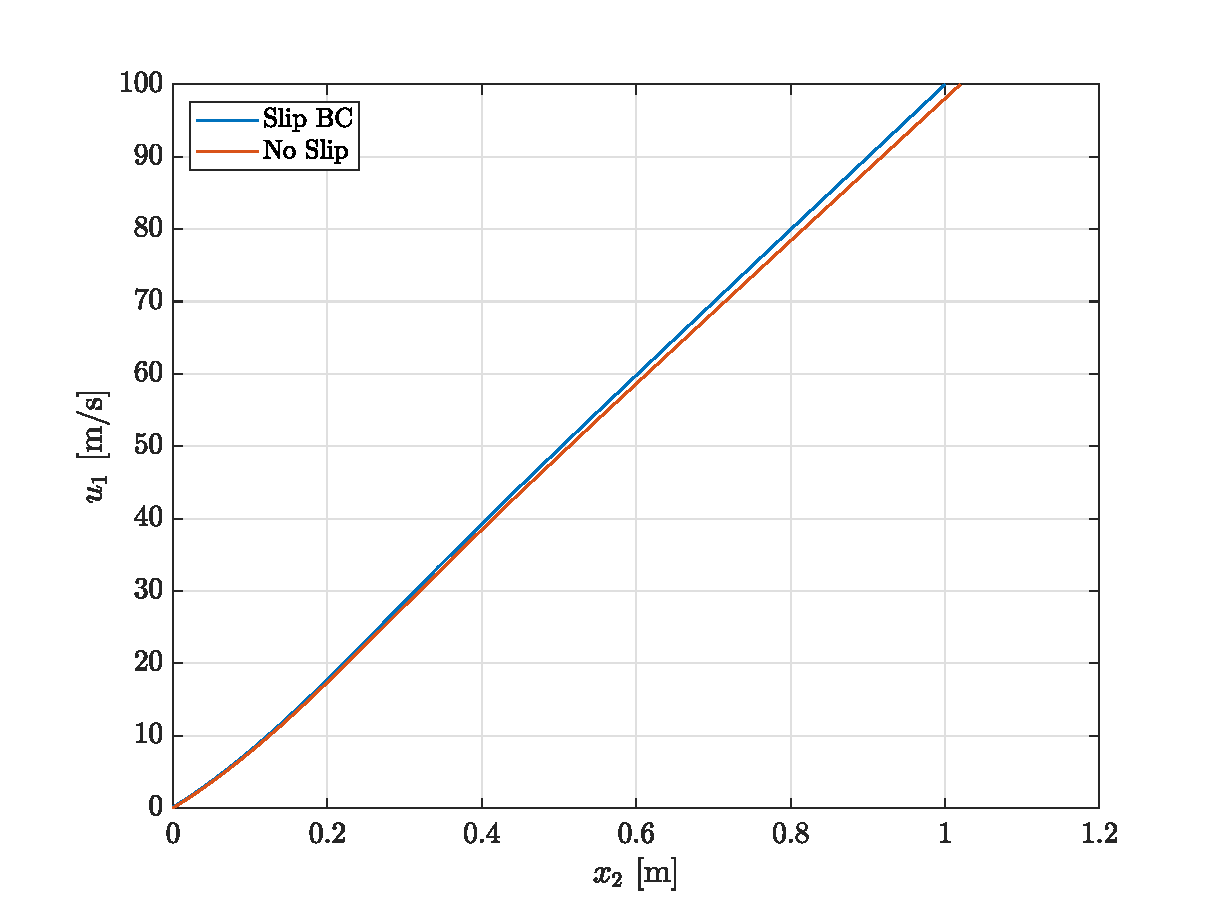
\includegraphics[width = \textwidth]{img/comp1.eps}
        \caption{Full velocity profile}
        \label{fig:plotnorm}
    \end{subfigure}
    \begin{subfigure}{0.45\textwidth}
        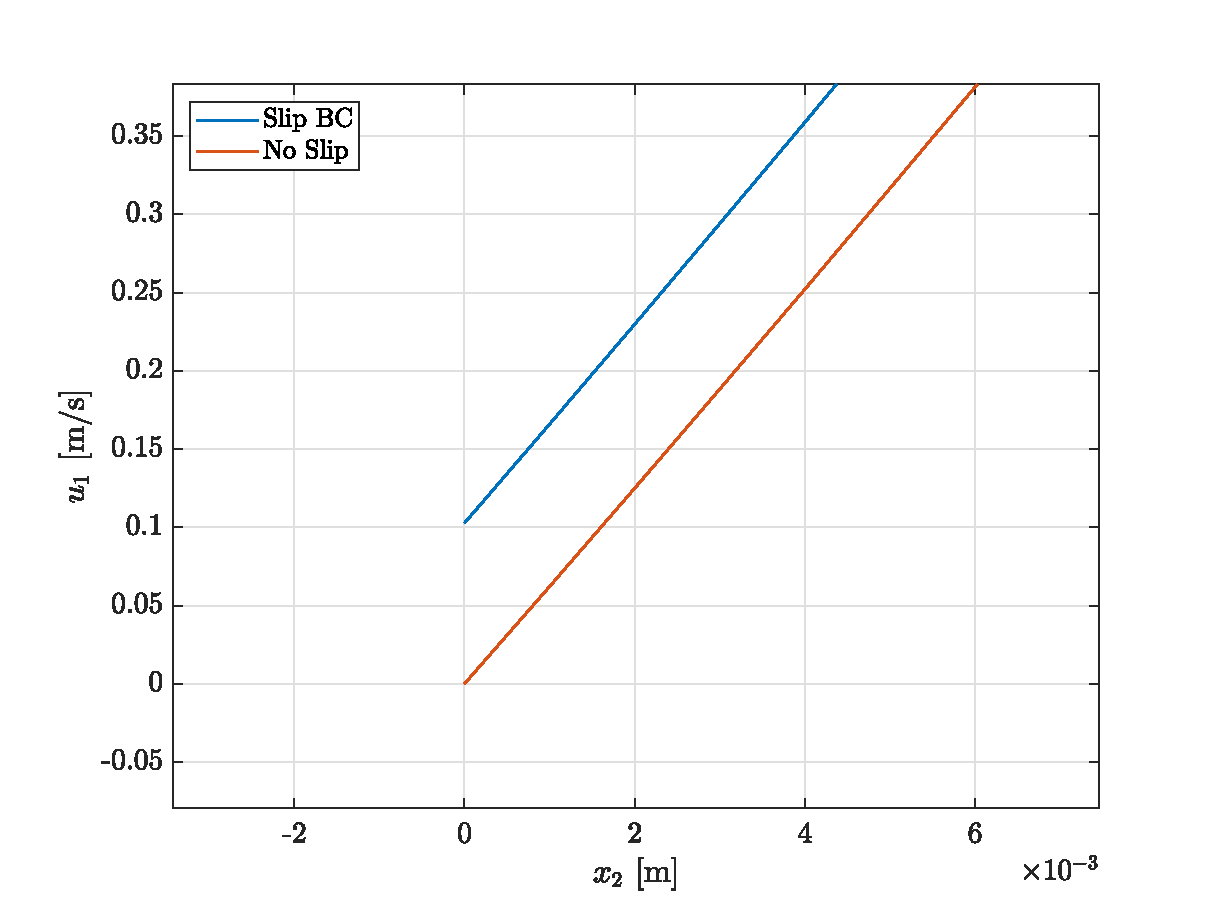
\includegraphics[width = \textwidth]{img/comp1_zoom.eps}
        \caption{Zoom of the velocity profile near the wall}
        \label{fig:plotzoom}
    \end{subfigure}
    \caption{Plot of the $u_1$ velocity component over a flat plate with and without slip boundary conditions}
    \label{fig:plot}
\end{figure}

\section{Conclusions and future work}

This project has shown the successful implementation of slip boundary conditions in PHASTA, as was intended. Additionally, both Dirichlet-type and Nitsche-type implementations of the 1D Maxwell model have been presented.

Having set the foundation with the subsonic case, the next step is to validate the results under hypersonic conditions corresponding to a spacecraft reentering Earth's atmosphere. To do that, the idea is to start simulations with a simple uniform flow over a flat plate, allowing for the shock to form at the edge (depending on the mesh, this might require the use of discontinuity capturing, available in PHASTA on the \texttt{e3DC \textit{(compressible/e3dc.f)}} routine), and then studying the behavior throughout the rest of the plate. 

This scenario is to be reproduced at multiple flight conditions equivalent to a spacecraft reentering Earth's atmosphere; that is, multiple Knudsen numbers (up to $\mathrm{Kn} \sim 1$), multiple Mach numbers, and multiple wall temperatures. At least some of these conditions will be selected in order to match other available data.

For the same range of conditions, simulations will also be run with the original PHASTA codebase in order to determine when and where the continuum breakdown happens. For that, the gradient-length local (GLL) Knudsen number \cite{boydSlip} will be used.

In order to validate the obtained results, the velocity and temperature profiles at the wall will be compared with both Direct Simulation Monte Carlo and Navier--Stokes simulations \cite{evaluation, gokcen1} and experiments \cite{boydExperiment, lockerbyCapturing} from other sources. Finally, skin friction coefficient and different integrated quantities ---such as total drag--- will be compared against DSMC simulations to be performed using the SPARTA software \cite{sparta}.

Further work would consist in the implementation of the generalized Maxwell condition, which was presented in \autoref{eq:generalized}. Doing this would allow for accurate simulations of bodies other than the basic 2D flat plate (in which case the generalized slip model reduces to the 1D version), including a simple sphere or a blunt cone under uniform flow, as both cases have been tested before and there is available data for validation \cite{computationBlunt, boydSlip, numerical, gokcen2}. These simulations would be interesting to see how the generalized Maxwell condition actually accounts for surface curvature.

\pagebreak

\ucbbib

\end{document}
